\chapter{Teoría de Lie y ecuaciones diferenciales}


\section{Introducción histórica}




\begin{quote}
<<Marius Sophus Lie fue un matemático noruego (17 de diciembre de 1842-18 de febrero de 1899) que creó en gran parte la teoría de la simetría continua, y la aplicó al estudio de la geometría y las ecuaciones diferenciales.
La herramienta principal de Lie, y uno de sus logros más grandes fue el descubrimiento de que los grupos continuos de transformación (ahora llamados grupos de Lie), podían ser
 entendidos mejor "linealizándolos", y estudiando los correspondientes campos vectoriales generadores (los, así llamados, generadores infinitesimales).
Los generadores obedecen una versión linealizada de la ley del grupo llamada el corchete o conmutador, y tienen la estructura de lo que hoy, en honor suyo, llamamos un álgebra de Lie.>>
\end{quote}
\marginpar{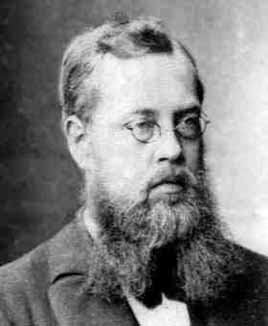
\includegraphics[scale=.28]{imagenes/Sophus_Lie.jpg}
}

\begin{flushright}
Wikipedia
\end{flushright}


 
\begin{quote}
<< La historia del análisis de simetrías comenzó a mediados del siglo XIX cuando S. Lie
Y F. Klein se reunieron en Berlín. Ambos matemáticos contribuyeron mucho a la teoría de las
simetrías. S. Lie presentó su famosa obra para examinar las simetrías en relación con
ecuaciones algebraicas y diferenciales. En su programa de Erlangen, Klein desarrolló las contrapartes discreta y algebraica de la aplicación de las simetrías a las funciones. S. Lie
creo un gran campo de las ecuaciones diferenciales, que fue muy útil para
clasificar las ecuaciones diferenciales de una forma nueva. La teoría desarrollada por Lie es
muy laboriosa, si se hace a mano. Esta es una de las razones por las que la aplicación de
esta teoría desapareció en la práctica de resolver problemas. Muy pocas personas usaron los procedimientos de  Lie para examinar ecuaciones diferenciales. Uno de ellos fue Birkhoff,
quien en la década de 1950 aplicó la teoría a problemas hidrodinámicos. En los últimos años,
 se prestó más atención a la teoría de Lie como uno de los métodos raros para obtener
soluciones, especialmente para ecuaciones diferenciales no lineales. Hoy el procedimiento de Lie es
accesible para su aplicación, si es usado el poder computacional del álgebra computacional. 
Los cálculos algebraicos muy extendidos hoy en día se llevan a cabo por computadoras. 
En los últimos 20 años, ha habido un enorme aumento de la potencia de  las computadoras y del desarrollo de lenguajes simbólicos, permitiendo abordar problemas en una
manera más sencilla.>>
\end{quote}
  

\begin{flushright}

Symmetry Analysis of
Differential Equations
with Mathematica\textregistered\\
\cite{GerdBaumann578}

\end{flushright}




\section{Cambios de Variables}

Vamos a seguir estudiando ecuaciones no lineales de primer orden

\boxedeq{\frac{dy}{dx}=f(x,y)}{eq:gral_orden1}
o, utilizando  la escritura en  \emph{forma diferencial}
\boxedeq{M(x,y)dx+N(x,y)dy=0.}{eq:gral_orden1_FormDif}
En el apéndice \ref{section:fromas} discutimos muy sumariamente el concepto de forma diferencial.

\begin{problema}[Cambio de variables]
 Dada la ecuación \eqref{eq:gral_orden1} o \eqref{eq:gral_orden1_FormDif} en las variables $x,y$. Queremos encontrar nuevas variables 
 \begin{equation}\label{eq:cambio_prin}
  \left \{\begin{array}{cc}
	    \hat{x}&=\hat{x}(x,y)\\
	    \hat{y}&=\hat{y}(x,y)
          \end{array}
 \right. .
 \end{equation}
tales que la ecuación se transforme en una que podamos resolver.
\end{problema}

Para no correr riesgos de perder información en la ecuación transformada, es conveniente que 
$x$ e $y$ también se expresan en función de $\hat{x}$ e $\hat{y}$, vale decir que la transformación pueda invertirse:
 \begin{equation}\label{eq:cambio_inv}
  \left \{\begin{array}{cc}
	    x&=x(\hat{x},\hat{y})\\
	    y&=y(\hat{x},\hat{y})
          \end{array}
 \right. .
 \end{equation}
\subsection{Cómputos de cambios de variables}\marginpar{Es costumbre recurrir a un abuso de notación que suele producir confusión al estudiante. Nos referimos a distinguir las derivadas $\partial y/\partial x$ y  $d y/d x$. Tratándose $y$ en el caso que nos ocupa, de una función de $x$ e $\hat{y}$,    la derivada $\partial y/\partial x$ representa la derivada parcial de $y$ respecto a su primera variable. Como $\hat{y}$ es a su vez función de $x$, por  $d y/d x$ denotamos la derivada de $y$ atendiendo a que la segunda variable también depende de $x$.}
Vamos a estudiar en primer lugar como computar cambios de variables. Empezaremos por casos más sencillos hasta ir a la situación más general.

\subsubsection{Cambio de la variable dependiente manteniendo la independiente}

 Supongamos que el conjunto de variables se relacionan  por las identidades $x=\hat{x}$ e  $y=y(x,\hat{y})$. Notar que en este caso usamos la relación inversa. Entoces, derivando $y$ respecto a $x$ y usando la regla de la cadena (que sería más apropiado llamarla regla de cambio de variables para la derivada)

\[\frac{dy}{dx}=\frac{\partial y}{\partial x}+\frac{\partial y}{\partial \hat{y}}\frac{d\hat{y}}{dx}.\]

La ecuación se convierte

\[\frac{\partial y}{\partial x}+\frac{\partial y}{\partial \hat{y}}\frac{d\hat{y}}{dx}=f(x,y(x,\hat{y})).\]
Que es una expresión sólo en $\hat{y}$ y $x$. Parece más complicada, pero en un ejemplo concreto puede ser más simple.







\begin{ejemplo} Hacer el cambio de variable propuesto en la  ecuación indicada
\[y=\frac{e^{\hat{y}}}{x}\quad\text{en}\quad  y'=\left[\ln(xy)\right]^2xy-\frac{y}{x}.\]
 1) Expresemos $dy/dx$ sólo con $x$, $\hat{y}$ y $d\hat{y}/dx$.
\[\frac{dy}{dx}=-\frac{e^{\hat{y}}}{x^2}+\frac{e^{\hat{y}}}{x}\frac{d\hat{y}}{dx}.\]
 2) Remplacemos $y'$ e $y$ en la ecuación
\[-\frac{e^{\hat{y}}}{x^2}+\frac{e^{\hat{y}}}{x}\frac{d\hat{y}}{dx}=\left[\ln\left(x \frac{e^{\hat{y}}}{x} \right)\right]^2x\frac{e^{\hat{y}}}{x}-\frac{\frac{e^{\hat{y}}}{x} }{x}.\]
 3) Simplifiquemos
\boxedeq{\frac{d\hat{y}}{dx}=\hat{y}^2x.}{}




\end{ejemplo}

\advertencia \emph{Importante:} Observar  que en un cambio de variable, ya se cambie la variable dependiente, independiente o ambas, las derivadas (tratándose de la velocidad de cambio de unas variables repecto a otras)  también hay que cambiarlas.


Podemos resolver los cambios de variables con \texttt{SymPy}, lo cual es muy útil por dos motivos. El primero porque nos permite hacer cambios de variables en expresiones muy grandes, resolviendo operaciones que a mano son sumamente tediosas. El segundo, y no menos importante para nosotros, es que es muy rico explorar un procedimiento enmarcándolo en un contexto muy distinto. En este caso, el procedimiento es relizar un cambio de variables y estamos explorando el mismo a través de un breve código que lo implementa en un lenguaje de programación.

\lstinputlisting[language=Python]{scripts/sust1.py}
\marginpar{
\begin{pspicture}(0,0)(1in,2in)
      %\rput(0,1){
      \scalebox{.7}{\psbarcode[file]{scripts/sust1.py}{}{qrcode}}
      %}
\end{pspicture}
}
Obtenemos la ecuación
\[\frac{1}{x} \left(- x \log^{2}{\left (e^{\operatorname{y\_n}{\left (x \right )
}} \right )} + \frac{d}{d x} \operatorname{y\_n}{\left (x \right )}\right) e^{
\operatorname{y\_n}{\left (x \right )}} = 0\]
que \texttt{SymPy} no simplifica a nuestro gusto




\subsubsection{Cambio de la variable independiente manteniendo la dependiente}

Supongamos  $\hat{x}=\hat{x}(x)$. Usamos la relación
\[\frac{dy}{dx}=\frac{dy}{d\hat{x}}\frac{d\hat{x}}{dx}.\]
Suponiendo que la relación $\hat{x}=\hat{x}(x)$ se invierte en $x=x(\hat{x})$, todo lo que resta es sustituir  $x$ por su igual en términos de $\hat{x}$

\[\frac{dy}{d\hat{x}}=f(x(\hat{x}),y) \left[\left.\frac{d\hat{x}}{dx}\right|_{x=x(\hat{x})}\right]^{-1}.\]
Que es una expresión sólo en $\hat{x}$ e $y$. Describir el procedimiento  en general puede hacer parecer que es más dificil de lo que en realidad es en un caso concreto.



\begin{ejemplo} Hacer el cambio de variable en la  ecuación indicados
\[x=\cos \hat{x}\quad\text{en}\quad  -\frac{dy}{dx}+\frac{x}{\sqrt{1-x^2}}y=0.\]
1) $\hat{x}=\arcsen x$
\[\frac{dy}{dx}=\frac{dy}{d\hat{x}} \frac{d\hat{x}}{dx}  =-\frac{1}{\sqrt{1-x^2}}\frac{dy}{d\hat{x}}.\]
 2) Remplacemos $x$ e $y'$ en la ecuación
\[\frac{1}{\sqrt{1-x^2}}\frac{dy}{d\hat{x}}+ \frac{x}{\sqrt{1-x^2}}y=0\]
3) Reemplazando $x$ por $\cos(\hat{x})$ y simplificando
\[\frac{dy}{d\hat{x}}+\cos(\hat{x}) y=0.\]

\end{ejemplo}


Para hacer esto con \texttt{SymPy} (de ahora en más omitiremos la sentencia de importanción del módulo, esta operación se hace sólo una vez por sesion).
\lstinputlisting[language=Python]{scripts/sust2.py}
\marginpar{
\begin{pspicture}(0,0)(1in,1in)
      %\rput(0,1){
      \scalebox{.7}{\psbarcode[file]{scripts/sust2.py}{}{qrcode}}
      %}
\end{pspicture}
}
Obtenemos la ecuación
\[\frac{y{\left (\operatorname{acos}{\left (\cos{\left (xn \right )} \right )} \right )} \cos{\left (xn \right )}}{\sqrt{- \cos^{2}{\left (xn \right )} + 1}}
+ \frac{1}{\sqrt{- \cos^{2}{\left (xn \right )} + 1}} \left. \frac{d}{d \xi_{1
}} y{\left (\xi_{1} \right )} \right|_{\substack{ \xi_{1}=\operatorname{acos}{
\left (\cos{\left (xn \right )} \right )} }}\]
Nuevamente \texttt{SymPy} no simplifica a nuestro gusto, esto ocurre aún con aquellas expresiones que parece muy evidente como se simplifican. El caso es que la operación de simplificación es por un lado  subjetiva, depende de un supuesto tácito de a que expresión se quiere arribar y por otro algunas expresiones, por ejemplo $\ln\exp(z)$, se simplifican en determinados campos numéricos y en otros no. En el caso del ejemplo $\ln\exp(z)$, la expresión es simplificable si $z\in\rr$, pero no lo es si por ejemplo $z\in\mathbb{C}$. De modo que no puede esperarse que Sympy efectúe esta simplificación a menos que conozca que se trabaja en el campo numérico indicado. Hay que distinguir que supuestos tácitos está haciendo uno y hay que indicarselos a Sympy.    El lector debe tener en cuenta que en ningún momento uno le dijo a \texttt{SymPy} que tipo de ente estaba manipulando en expresiones del tipo \texttt{x\_n=acos(x)}. Puede parecer natural que se trata de números reales, no obstante esta 
información nunca fue comunicada al interprete de \texttt{SymPy}. ¿Porqué el habría de entender que \texttt{x} es real? Si al fin y al cabo \texttt{x\_n=acos(x)} tiene sentido si \texttt{x} es complejo y aún si es una matríz. Muchas veces las operaciones que se simplifican en un campo no lo pueden hacer en otro. El comando  \texttt{symbols} tiene la opción de informar a \texttt{SymPy} que tipo de ente representa \texttt{x} de la siguiente forma
\texttt{x=symbols('x',real=True)}. De esta forma se consiguen mejores resultados en las simplificaciones.


\subsubsection{Cambio de variable general $\hat{x}=\hat{x}(x,y)$, $\hat{y}=\hat{y}(x,y)$}
\begin{enumerate}
  \item Calculamos $d\hat{y}/d\hat{x}$ en las variables $x,y$
    \boxedeq{
      \frac{d\hat{y}}{d\hat{x}}=\frac{\frac{d\hat{y}}{dx}}{\frac{d\hat{x}}{dx}}=\frac{\frac{\partial\hat{y}}{\partial x}+\frac{\partial\hat{y}}{\partial y}y'}{\frac{\partial\hat{x}}{\partial x}+\frac{\partial\hat{x}}{\partial y}y'}=\frac{\frac{\partial\hat{y}}{\partial x}+\frac{\partial\hat{y}}{\partial y}f(x,y)}{\frac{\partial\hat{x}}{\partial x}+\frac{\partial\hat{x}}{\partial y}f(x,y)}.
	    }{eq:subsder}

   \item En la expresión resultante sustituímos $x,y$ por las tansformaciones 			inversas $x=x(\hat{x},\hat{y})$ y  $y=y(\hat{x},\hat{y})$
\end{enumerate}



\begin{ejemplo}\label{ej:cambio_forma} Transformar a polares
 \[
  \frac{dy}{dx}=\frac{y^3+x^2y-x-y}{x^3+xy^2-x+y}.
 \]
\end{ejemplo}

Dado que el cálculo es extenso lo haremos con \texttt{SymPy}, el procedimiento seguido ilustra como hacerlo a mano. Es ilustrativo hacer esto último para apreciar la utilidad de usar un sistema de álgebra computacional (SAC) como \texttt{SymPy}.

\lstinputlisting[language=Python]{scripts/sust3.py}
\marginpar{
\begin{pspicture}(0,-.5)(1in,1in)
      %\rput(0,1){
      \scalebox{.7}{\psbarcode[file]{scripts/sust3.py}{}{qrcode}}
      %}
\end{pspicture}
}

Obtenemos la siguiente expresión 
\[\frac{dr}{d\theta}=\frac{\frac{dr}{dx}}{\frac{d\theta}{dx}}=\frac{\left(1 + \frac{1}{x^{2}} y^{2}{\left (x \right )}\right) \left(x + y{\left (x \right )} \frac{d}{d x} y{\left (x \right )}\right)}{\sqrt{x^{2} + y^{2}{\left (x \right )}} \left(\frac{1}{x} \frac{d}{d x} y{\left (x \right )} - \frac{1}{x^{2}} y{\left (x \right )}\right)}.\]
Ahora sustituímos $y'(x)$ usando la ecuación diferencial, redefinimos $r,\theta$ fundamentalmente para limpiar el valor que tenían asignado en el código previo, que era una expresión de $x,y$, y finalmente sustituímos $x$ e $y$ por su expresión en polares.

\lstinputlisting[language=Python]{scripts/sust4.py}
\marginpar{
\begin{pspicture}(0,-.5)(1in,1in)
      %\rput(0,1){
      \scalebox{.6}{\psbarcode[file]{scripts/sust4.py}{}{qrcode}}
      %}
\end{pspicture}
}
 Encontramos que en polares la ecuación es mucho más simple
\[\frac{dr}{d\theta}=-r^3+r.\]

 Quizás  usar la notación como  forma diferencial sea más efectivo. Como $r$ y $\theta$ son funciones de $x$ e $y$, ellas son 0-formas. Usando las reglas de la diferencial, hay que reemplazar
\[
\begin{array}{ll}
x=r\cos\theta; &dx=\cos\theta dr-\sen\theta r d\theta\\
 y= r\sen\theta; & dy=\sen\theta dr+\cos\theta r d\theta\\
\end{array}
\]
en la 1-forma:
\[(y^3+x^2y-x-y)dx-(x^3+xy^2-x+y)dy.\]

Sympy posee un módulo para operar con formas diferenciales, en un apéndice describimos como utilizarlo para resolver este ejemplo.

\section{Grupos}

\marginpar{Las raíces históricas de la teoría de grupos son la teoría de las ecuaciones algebraicas, la teoría de números y la geometría. Euler, Gauss, Lagrange, Abel y Galois fueron los creadores que ponen los cimientos de esta rama del álgebra abstracta.  Otros importantes matemáticos que contribuyen son Cayley, Emil Artin, Emmy Noether, Peter Ludwig Mejdell Sylow, A.G. Kurosch, Iwasawa entre muchos otros.
\raggedright{(Wikipedia)}
}
 \subsection{Definición y ejemplos}
\begin{definicion}[Grupo]
Un \href{https://es.wikipedia.org/wiki/Grupo_(matem%C3%A1tica)}{grupo} es un par $(G,\cdot)$ donde $G$ es un conjunto y $\cdot :G\times G\to G$ una \href{https://es.wikipedia.org/wiki/Operaci%C3%B3n_matem%C3%A1tica}{operación binaria interna} que satisface
\begin{enumerate}
\item $(g_1\cdot g_2)\cdot g_3=g_1\cdot (g_2\cdot g_3)$, para todos $g_1,g_2,g_3\in G$,
\item Existe $e\in G$ tal que $e\cdot g=g\cdot e=g$,  para todo $g\in G$.
\item Para todo $g\in G$ existe $h\in G$ tal que $g\cdot h=h\cdot g=e$. Esta función $h$ se denota  $g^{-1}$.
\end{enumerate}
\end{definicion}

Es usual omitir el punto para indicar la operación, i.e. escribimos $g\cdot h=gh$.



\begin{ejemplo} Sea $\Pi$ un plano euclideano y $G$ el conjunto de todas las transformaciones rígidas de $\Pi$ en si mismo. Entonces $G$ es un grupo con la operación de composición. Se llama el \emph{grupo de transformaciones rígidas}.
 \end{ejemplo}


\begin{ejemplo}  Sea $X=\{x_1,\ldots,x_n\}$ un conjunto de $n$ elementos y $S_n$ definido por
\[S_n=\{\sigma|\sigma:X\to X\hbox{ y }\sigma \hbox{ es biyectiva }\}\]
Entonces $S_n$ es un grupo  con la operación de composición. Se denomina \href{http://es.wikipedia.org/wiki/Grupo_simétrico}{\emph{grupo simétrico}}.
 \end{ejemplo}

\begin{ejemplo} Sea $\Delta$ un polígono regular de $n$ lados  en un plano euclideano $\Pi$ y $D_{2n}$ el conjunto de todas las transformaciones rígidas de $\Pi$ en si mismo que llevan $\Delta$ en si mismo. $D_{2n}$ se llama el \href{http://es.wikipedia.org/wiki/Grupo_diedral}{\emph{grupo diedral}}  de orden $2n$. Para un triángulo equilatero:
\begin{center}
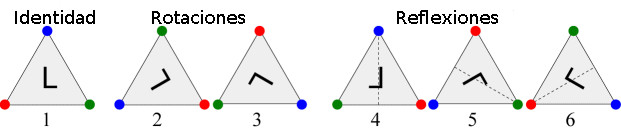
\includegraphics[scale=.4]{imagenes/SimTria.jpg}
\end{center}
\end{ejemplo}

Recordemos el siguiente concepto.

\begin{definicion}[Acción de un grupo sobre un conjunto]
Diremos que un grupo $G$ actúa sobre el conjunto $X$ si existe una operación binaria externa  $\star:G\times X\to G$ que satisface:
\begin{enumerate}
\item Si $e$ es el neutro de $G$, $e \star x=x$,  para todo $x\in X$.
\item Para todos $g,h\in G$ y $x\in X$,    $g\star (h\star x)=(gh)\star x$.
\end{enumerate}
\end{definicion}

Como en el caso de grupos suele nos escribirse el símbolo de la operación binaria, i.e. se escribe $g\star x= gx$.




\section{Grupos continuos de simetrías}

\subsection{Grupos y cambios de variables}

Los cambios de variables de un conjunto de dos variables, digamos $x$ e $y$, son funciones $\Gamma$, invertibles,  de clase $C^1$, donde $\Gamma:\Omega_1\to\Omega_2$, con $\Omega_1,\Omega_2$ abiertos de $\rr^2$.  Acostumbraremos escribir $(\hat{x},\hat{y})=\Gamma(x,y)$ y diremos que $(\hat{x},\hat{y})$ son la variables nuevas y $(x,y)$ las viejas.

\begin{ejemplo} \textbf{Coordenadas polares.} Es más facil describir la transformación que lleva coordenadas polares en cartesianas. En este caso $(x,y)=\Gamma(r,\theta)$ y
\[
\begin{array}{ll}
\Gamma(r,\theta)&=(r\cos(\theta),r\sen(\theta)),\\
\Omega_1&=(0,\infty)\times (-\pi,\pi),\\
\Omega_2&=\rr^2-\{(x,y)|y=0,x\leq 0\}\\
\end{array}
\]
\end{ejemplo}

\subsection{Grupos de Lie uniparamétricos}

\begin{definicion}[Grupos de Lie uniparamétricos]  Supongamos dada una acción del grupo  $(\rr,+)$ en $\rr^2$. En este caso vamos a adoptar una notación funcional, i.e. en lugar de escribir $\epsilon\star (x,y)$, con $\epsilon\in\rr$ y $(x,y)\in\rr^2$ pondremos $\Gamma_{\epsilon}(x,y)$. Denotaremos por $\{\Gamma_{\epsilon}\}$ a la acción introducida.  Notar que $\{\Gamma_{\epsilon}\}$  satisface que 
\begin{enumerate}
 \item $\forall\epsilon_1,\epsilon_2\in\rr:\Gamma_{\epsilon_1}\circ \Gamma_{\epsilon_2}=\Gamma_{\epsilon_1+\epsilon_2}$.

\item $\Gamma_0=I$.

\item $\Gamma_{\epsilon}$ es invertible y $\left(\Gamma_{\epsilon}\right)^{-1}=\Gamma_{-\epsilon}$
\end{enumerate}

La acción $\Gamma_{\epsilon}$ se denomina un  \href{http://es.wikipedia.org/wiki/Grupo_uniparamétrico}{\emph{grupo de Lie uniparamétrico}} si además:

\begin{enumerate}
\item[4.] $\forall\epsilon\in\rr:\Gamma_{\epsilon}$ es un difeomorfismo sobre $\rr^2$.


\item[5.] Si $\Gamma_{\epsilon}(x,y)=\left(\hat{x}(x,y,\epsilon),\hat{y}(x,y,\epsilon)\right)$ entonces   las funciones  $\hat{x}(x,y,\epsilon)$ y $\hat{y}(x,y,\epsilon)$  se desarrollan en serie de potencias respecto a $\epsilon$. Es decir para todo $\epsilon_0\in\rr$ existen coeficientes $a_j$ y $b_j$, $j=0,1,\ldots$, y $r>0$ tales que
\begin{equation}\label{eq:des_serie}
\begin{array}{cc}
\hat{x}(x,y,\epsilon)&=a_0(x,y)+a_1(x,y)(\epsilon- \epsilon_0)+\cdots\\
\hat{y}(x,y,\epsilon)&=b_0(x,y)+b_1(x,y)(\epsilon- \epsilon_0)+\cdots\\
\end{array}
\end{equation}
para $|\epsilon-\epsilon_0|<r$.
\end{enumerate}
\end{definicion}



\begin{ejemplo} Demostrar que las siguientes aplicaciones inducen grupos de Lie uniparamétricos
\begin{enumerate}
\item $\Gamma_{\epsilon}(x,y)=(x+\epsilon,y)$ y $\Gamma_{\epsilon}(x,y)=(x,y+\epsilon)$.
\item $\Gamma_{\epsilon}(x,y)=(e^{\epsilon}x,y)$
\item$\Gamma_{\epsilon}(x,y)=\left(\frac{x}{1-\epsilon x},\frac{y}{1-\epsilon x} \right)$
\item$\Gamma_{\epsilon}(x,y)=\begin{pmatrix} \cos(\epsilon) & -\sen(\epsilon)
\\ \sen(\epsilon) & \cos(\epsilon)
\end{pmatrix} \begin{pmatrix} x\\ y
\end{pmatrix}
$
\end{enumerate}
\end{ejemplo}

Vamos a desarrollar sólo el ejemplo de $\Gamma_{\epsilon}(x,y)=(x+\epsilon,y)$. La propiedad 1 en la definición la chequearemos con  \texttt{SymPy}. 
\marginpar{
\begin{pspicture}(0,3)(1in,1in)
      %\rput(0,1){
      \scalebox{.5}{\psbarcode[file]{scripts/prop_grupo.py}{}{qrcode}}
      %}
\end{pspicture}
}
 \lstinputlisting[language=Python]{scripts/prop_grupo.py}

 La propiedad 2 en la definición es evidente y la propiedad 3 es siempre consecuencia de 1. y 2. 
Se incluyó en la lista sólo para resaltar su cumplimiento, pero no es necesario chequearla. La propiedad 4. es clara la 5. también lo es, notar que el desarrollo en serie \eqref{eq:des_serie} es válido en este caso con $a_0(x,y)=x$, $a_1(x,y)=1$, $a_j(x,y)=0$, $j\geq 2$, $b_0(x,y)=y$ y $b_j(x,y)=0$, $j\geq 1$. La justificaciones correspondientes al resto de los ejemplos queda como ejercicio.\actividad


 Las reflexiones en el plano, por ejemplo $\Gamma(x,y)=(-x,y)$,  no pueden  pertenecer a un  grupo de Lie uniparamétrico. Más generalmente:
 
 \begin{teorema}
   Una transformación  $T:\rr^2\to\rr^2$ tal que el determinante de la matriz Jacobiana $\det(DT)$ sea negativo en algún punto no puede pertenecer a un grupo de Lie uniparamerico. Dicho de otro modo, debe ocurrir que $\det(D\Gamma_{\epsilon})>0$ para todo $\epsilon$ y todo grupo $\{\Gamma_{\epsilon}\}$.
 \end{teorema}
\begin{proof}
 Si $\Gamma_{\epsilon}$ es un grupo y supongamos por ejemplo que existe $\epsilon_0\in\rr$ y $(x_0,y_0)\in\rr^2$ tal que:

\[J(x_0,y_0,\epsilon_0):=\det\begin{pmatrix} \frac{\partial\hat{x}}{\partial x}&  \frac{\partial\hat{x}}{\partial y}\\
 \frac{\partial\hat{y}}{\partial x} &  \frac{\partial\hat{y}}{\partial y}\\
\end{pmatrix}<0,
\]
donde las derivadas son tomadas en $\epsilon=\epsilon_0, x=x_0$ y $y=y_0$.
 Por otro lado tenemos que $J(x_0,y_0,0)=1$. Como $J(x_0,y_0,\epsilon)$ es continua respecto a $\epsilon$ debería existir $\epsilon'$ con $J(x_0,y_0,\epsilon')=0$. Esto implica que la matriz jacobiana $D\Gamma_{\epsilon}$ es singular y esto contradice que $\Gamma:\rr^2\to \rr^2$ es difeomorfismo ($D\Gamma D\Gamma^{-1}=I$).
\end{proof}


 
 
 



 En el caso de la reflexión $\Gamma(x,y)=(x,-y)$, se  genera un grupo discreto, ya que $\Gamma^2=\Gamma\circ \Gamma=I$. Luego $\Gamma$ genera el grupo finito $G=\{I,\Gamma\}$ que es isomorfo a $\mathbb{Z}_2$. En este caso diremos que    $\{I,\Gamma\}$ es un \emph{grupo discreto}.





\subsection{Grupos de simetrías de EDO}
\begin{definicion}[Grupo de simetrías de una ecuación]
 Consideremos una ecuación
\boxedeq{y'=f(x,y).}{eq:principi}
Una transformación o cambio de variables $\Gamma$ se denomina una \emph{simetría} de la ecuación si el cambio de variables dado por $(\hat{x},\hat{y})=\Gamma(x,y)$ deja invariante  la ecuación.  Diremos que un grupo de Lie uniparamétrico $\{\Gamma_{\epsilon}\}$ es un grupo uniparamétrico de simetrías de \eqref{eq:principi} si $\Gamma_{\epsilon}$ es simetría de la ecuación para cada $\epsilon$.

\end{definicion}


De acuerdo con \eqref{eq:subsder} para que $(\hat{x},\hat{y})=\Gamma(x,y)$ sea una simetría de \eqref{eq:principi} se debe cumplir que
 \boxedeq{\frac{\frac{\partial\hat{y}}{\partial x}+\frac{\partial\hat{y}}{\partial y}f(x,y)}{\frac{\partial\hat{x}}{\partial x}+\frac{\partial\hat{x}}{\partial y}f(x,y)}=f(\hat{x},\hat{y})}{eq:cond_sim}

 Esta ecuación se llama \emph{condición de simetría}. Es una ecuación en derivadas parciales, en principio más compleja que la ecuación original. Tiene varios grados de libertad, por lo que suele haber muchas simetrías.  Es común que encontremos soluciones a  traves de un  \href{http://es.wikipedia.org/wiki/Ansatz}{ansatz}.\link





 \begin{ejemplo} Consideremos la ecuación
   \begin{equation}\label{eq:trivial}y'=0.
    \end{equation}
    \begin{wrapfigure}[10]{r}{5.5cm}
   \vspace{-.5cm}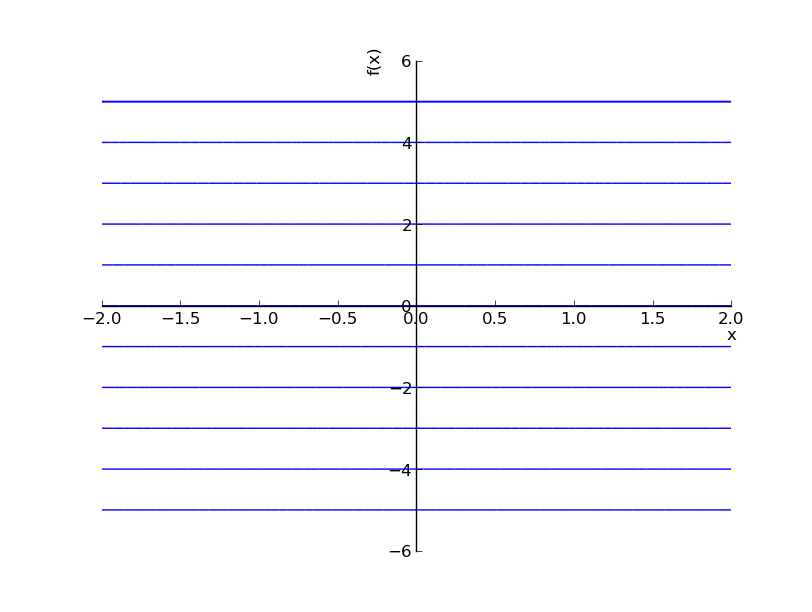
\includegraphics[scale=.3]{imagenes/sol_trivial.png}
 \end{wrapfigure}
La condición de simetría se reduce a 
\[
\frac{\frac{\partial\hat{y}}{\partial x}}{\frac{\partial\hat{x}}{\partial x}}=0
\]
Debemos tener que $\frac{\partial\hat{y}}{\partial x}=0$. Vale decir $\hat{y}$ es independiente de $x$. De allí la forma general de una simetría es 
\[\hat{x}=\hat{x}(x,y)\quad \hat{y}=\hat{y}(y).\]
\end{ejemplo}
 Hay muchas simetrías. Las traslaciones en cualquier dirección $(x,y)\mapsto (x+\alpha ,y+\beta)$ ($\alpha,\beta\in\rr$). Cambios de escala en ambos ejes  $(x,y)\mapsto (e^{\epsilon}x,y)$, $(x,y)\mapsto (x,e^{\epsilon}y)$. Reflexiones respecto ambos ejes  $(x,y)\mapsto (-x,y)$, $(x,y)\mapsto (x,-y)$.  Observar que el gráfico de las soluciones posee las mismas simetrías, pues en general \emph{las simetrías de una ecuación llevan soluciones en soluciones}.

 De todas las simetrías encontradas $\Gamma_{\epsilon}(x,y)=(e^{\epsilon}x,y)$, $\Gamma_{\epsilon}(x,y)=(x+\epsilon,y)$ y  $\Gamma_{\epsilon}(x,y)=(x+\epsilon,y)$ se llaman \emph{triviales} pues llevan una curva solución en si misma.  Cualquier cambio de la forma $\hat{x}=\hat{x}(x,y)\quad \hat{y}=y$ es trivial. \emph{Estamos interesados en hallar grupos de Lie uniparamétricos de simetrías no triviales.}




 \begin{ejemplo} Hallar simetrías de
\[\frac{dy}{dx}=f(x).\]
\end{ejemplo}
De acuerdo con \eqref{eq:subsder} se debe cumplir que
 \[\frac{\frac{\partial\hat{y}}{\partial x}+\frac{\partial\hat{y}}{\partial y}f(x)}{\frac{\partial\hat{x}}{\partial x}+\frac{\partial\hat{x}}{\partial y}f(x)}=f(\hat{x})\]
La forma de la ecuación sugiere el  \href{http://es.wikipedia.org/wiki/Ansatz}{ansatz}
   \[\boxed{\hat{x}=x},\quad \frac{\partial\hat{y}}{\partial x}=\frac{\partial\hat{x}}{\partial y}=0,\quad
   \frac{\partial\hat{y}}{\partial y}=\frac{\partial\hat{x}}{\partial x}. \]
 Luego 
\[\frac{\partial\hat{y}}{\partial y}=1\Rightarrow \boxed{\hat{y}=y+\epsilon} \]
con $\epsilon$ constante arbitraria. Hallamos que
\[\Gamma_{\epsilon}(x,y)=(x,y+\epsilon)\]
es un grupo de Lie uniparamétrico de simetrías. De manera similar
\[\Gamma_{\epsilon}(x,y)=(x+\epsilon,y)\]
es un grupo uniparamétrico de simetrías para 
\[\frac{dy}{dx}=f(y).\]
Geométricamente en el primer caso todas las soluciones se obtienen trasladando una cualquiera verticalmente y en el segundo caso horizontalmente.



\begin{tabular}{cc}
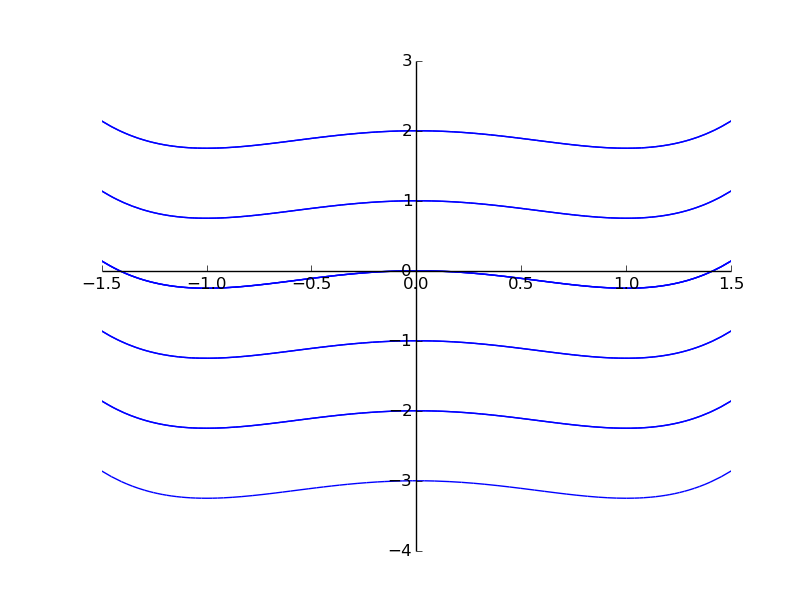
\includegraphics[scale=.3]{imagenes/sol_paralelas.png} &\hspace{-1.5cm}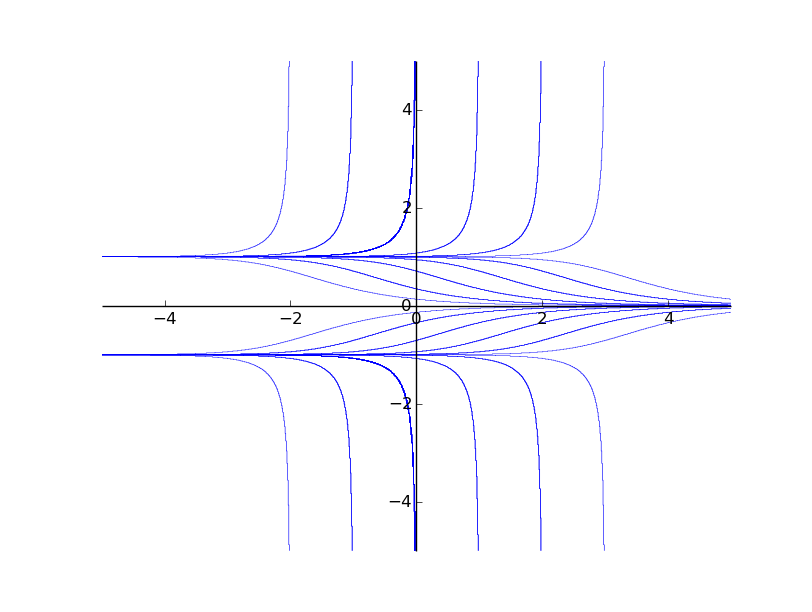
\includegraphics[scale=.3]{imagenes/sol_paralelas2.png} \\
Soluciones de $y'=x^3-x$ &\hspace{-1.5cm}Soluciones de $y'=y^3-y$
\end{tabular}





\begin{ejemplo}
 Demostrar que las rotaciones alrededor del origen es un grupo de Lie uniparamétrico de simetrías de
 \[\frac{dy}{dx}=\frac{y^3+x^2y-x-y}{x^3+xy^2-x+y}.\]
\end{ejemplo}
Sea $\Gamma_{\epsilon}$ la transformación que rota un ángulo $\epsilon$ alrededor del origen. Es un ejercicio demostrar que  $\{\Gamma_{\epsilon}|\epsilon\in\rr\}$ es un grupo uniparamétrico de simetrías. Se tiene la representación matricial
\[
\Gamma_{\epsilon}(x,y)= \begin{pmatrix} \hat{x}\\ \hat{y}
\end{pmatrix}=\begin{pmatrix} \cos(\epsilon) & -\sen(\epsilon)
\\ \sen(\epsilon) & \cos(\epsilon)
\end{pmatrix} \begin{pmatrix} x\\ y
\end{pmatrix}
\]

\[
\Gamma^{-1}_{\epsilon}(\hat{x},\hat{y})= \begin{pmatrix} x\\ y
\end{pmatrix}=\begin{pmatrix} \cos(\epsilon) & \sen(\epsilon)
\\ -sen(\epsilon) & \cos(\epsilon)
\end{pmatrix} \begin{pmatrix} \hat{x}\\ \hat{y}
\end{pmatrix}
\]


Para el cálculo recurrimos a \texttt{SymPy} (usamos \texttt{x\_n} en lugar de $\hat{x}$)
\marginpar{
\begin{pspicture}(0,5)(1in,1in)
      %\rput(0,1){
      \scalebox{.5}{\psbarcode[file]{scripts/sim_ecua1.py}{}{qrcode}}
      %}
\end{pspicture}
}e
 \lstinputlisting[language=Python]{scripts/sim_ecua1.py}




\begin{wrapfigure}[15]{r}{5.5cm}
 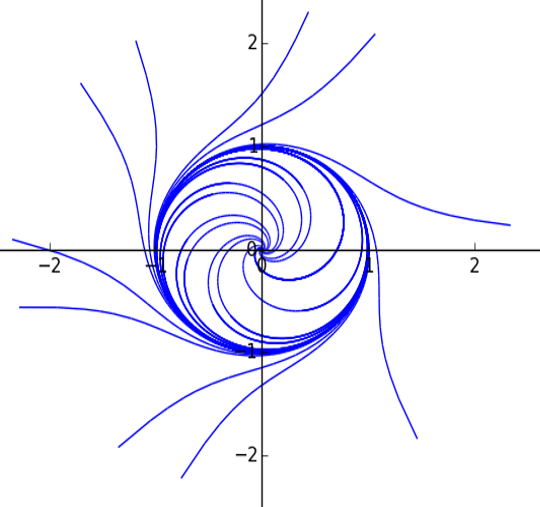
\includegraphics[scale=.4]{imagenes/sol_rotadas.png}
\end{wrapfigure}
La ecuación resultante es \emph{la misma}
\[\frac{dy_n}{dx_n}=\frac{x_{n}^{2} y_{n} - x_{n} + y_{n}^{3} - y_{n}}{x_{n}^{3} + x_{n} y_{n}^{2}
    - x_{n} + y_{n}}.\]
A la misma conclusión arribábamos si recordabamos que en en coordenadas polares la ecuación se escribe
\[\frac{dr}{d\theta}=r-r^3,\]
y que esta ecuación tiene las simetrías $\Gamma_{\epsilon}:(r,\theta)\mapsto (r,\theta+\epsilon)$. Si rotamos un ángulo fijo el gráfico de una solución obtenemos el gráfico de otra solución.








\begin{ejemplo}\label{ejem:tras} Supongamos que $y'=f(x,y)$ tiene  el grupo de Lie uniparamétrico de simetrías
\boxedeq{(\hat{x},\hat{y})=\Gamma_{\epsilon}(x,y)=(x,y+\epsilon)}{eq:tras_lie}
Usando la condición de simetrías \eqref{eq:cond_sim} tenemos
\[f(x,y)=f(\hat{x},\hat{y})=f(x,y+\epsilon).\]
La igualdad vale para todo $\epsilon$, luego poniendo $\epsilon=-y$ vemos que $f(x,y)=f(x,0):=f(x)$. Vale decir que $f$ es independiente de $y$ y la ecuación
\[y'=f(x),\]
se resuelve simplemente integrando.
\end{ejemplo}



\section{Órbitas, tangentes y curvas invariantes}


\begin{definicion}[Órbitas] Dado un grupo uniparamétrico de simetrías $G=\{\Gamma_{\epsilon}|\epsilon\in\rr\}$, y $(x_0,y_0)\in\rr^2$ llamamos \emph{órbita $(x_0,y_0)$ bajo la acción de  $G$} (simplemente órbita si es claro quien es $G$) a la curva
\[\{\Gamma_{\epsilon}(x_0,y_0)|\epsilon\in\rr\} \]
\end{definicion}

\begin{wrapfigure}[15]{r}{5.5cm}
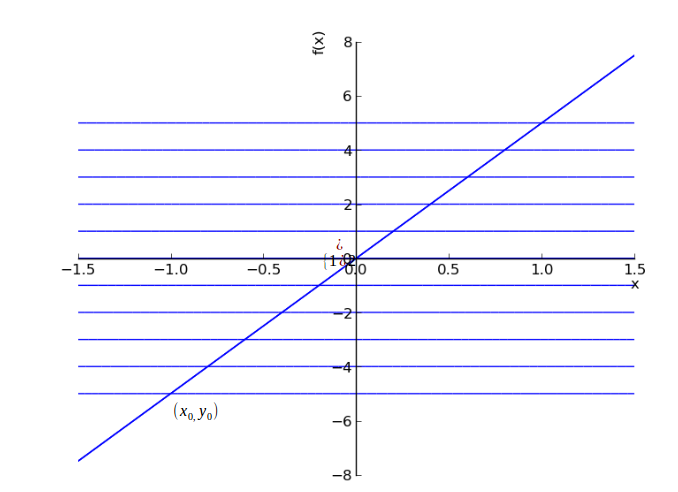
\includegraphics[scale=.3]{imagenes/sol_trivialB.png}
\end{wrapfigure}
Si $G$ es un grupo de simetrías no trivial, entonces es de esperar que la órbita de  $(x_0,y_0)$ cruce transversalmente las curvas solución. La órbita se usará como una nueva coordenada.
 La órbita atraves de $(x,y)$ es el conjunto de puntos de coordenadas
\begin{equation}\label{eq:orb} (\hat{x}(x,y,\epsilon),\hat{y}(x,y,\epsilon))=\Gamma_{\epsilon}(x,y),
\end{equation}
donde
\[(\hat{x}(x,y,0),\hat{y}(x,y,0))=(x,y).\]
Las ecuaciones \eqref{eq:orb} son ecuaciones parámetricas (parámetro $\epsilon$) de una  curva en el plano.

\begin{definicion}[Puntos invariantes]
Un punto $(x,y)$ se llama invariante si su órbita se reduce a $\{(x,y)\}$, vale decir
\[(x,y)=\Gamma_{\epsilon}(x,y),\quad\forall \epsilon>0\]
\end{definicion}






\begin{ejemplo} La órbita de $(x,y)$ bajo la acción del grupo  de Lie uniparamétrico
\[
\Gamma_{\epsilon}(x,y)= \begin{pmatrix} \hat{x}\\ \hat{y}
\end{pmatrix}=\begin{pmatrix} \cos(\epsilon) & -\sen(\epsilon)
\\ \sen(\epsilon) & \cos(\epsilon)
\end{pmatrix} \begin{pmatrix} x\\ y
\end{pmatrix}
\]
Son circunsferencias con centro en el origen. El punto $(0,0)$ es invariante.

\end{ejemplo}


\begin{definicion}[Campo vectorial de tangentes]
 Dado un grupo de Lie uniparamétrico $(\hat{x}(x,y,\epsilon),\hat{y}(x,y,\epsilon))=\Gamma_{\epsilon}(x,y)$  definimos el campo vectorial
\[(\xi(x,y),\eta(x, y))=\left(\left.\frac{d\hat{x}}{d\epsilon}\right|_{\epsilon=0}, \left.\frac{d\hat{y}}{d\epsilon}\right|_{\epsilon=0}   \right).\]
 $\xi$ y $\eta$ se llaman \emph{símbolos infinitesimales}.
 
 
Como $\hat{x},\hat{y}$ eran analíticas respecto a $\epsilon$ tenemos las fórmulas.

 
 \begin{equation}\label{eq:des_serie_infi}
\begin{array}{cc}
\hat{x}&=x+\epsilon\xi(x,y)+O(\epsilon^2)\\
\hat{y}&=y+\epsilon\eta(x,y)+O(\epsilon^2)\\
\end{array}
\end{equation}
 En un punto invariante \fbox{$\xi(x,y)=\eta(x,y)=0$}.
 
\end{definicion}





\begin{ejemplo}
Campo vectorial de infitesimales para las rotaciones. 
\end{ejemplo}
\begin{figure}[h]
 \begin{center}
  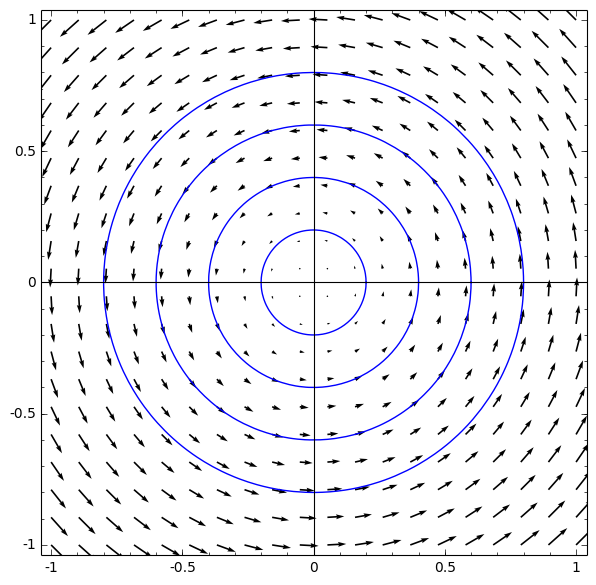
\includegraphics[scale=.3]{imagenes/CampoVectorial.png}
 \end{center}
\caption{Campo vectorial de infinitesimales $(\xi,\eta)$ }
\end{figure}

\begin{definicion}
 Más generalmente, un conjunto $C\subset\rr^2$ se dice \emph{invariante} por un grupo uniparamétrico de 
simetrías de Lie $\Gamma_{\epsilon}$ si y sólo si $\forall \epsilon: \Gamma_{\epsilon}(C)\subset C$, i.e. las órbitas de puntos en $C$ permanecen en $C$.
\end{definicion}

\noindent\textbf{Observaciones}
\begin{enumerate}
\item El conjunto unitario $\{(x,y)\}$ es invariante si y sólo si el punto $(x,y)$ 
es invariante.

\item Se $C$ es una curva plana suave, supongamos que $C$ viene dada por la ecuación implícita $g(x,y)=0$, con $\nabla g\neq 0$.  Supongamos que  $(\xi,\eta)\neq (0,0)$ sobre $C$. Entonces $C$ es invariante si y sólo si la tangente a  $C$ en cada punto $(x,y)$ es
paralela a $(\xi(x,y),\eta(x,y))$. La demostración de este hecho se propone como ejercicio. \actividad
\item Si en particular $C$ es una curva que viene descripta como el gráfico de una función $y=h(x)$, entonces $C$ es invariante si y sólo si
\boxedeq{Q(x,y,y')=\eta(x,y)-h'\xi(x,y)\equiv 0.}{eq:inv}
En efecto, en este caso $g(x,y)=y-h(x)$ (notar que $\nabla g=(-h'(x),1)\neq 0$). Como $\nabla g$ es perpendicular a $C$ tenemos la ecuación \eqref{eq:inv}. La ecuación \eqref{eq:inv} se llama \emph{ecuación característica}.


% \begin{definicion}[Curvas invariantes]
% Una curva plana $C$ se dice invariante por un grupo uniparamétrico de simetrías de Lie si y sólo si la tangente a  $C$ en cada punto $(x,y)$ es paralela a $(\xi(x,y),\eta(x,y))$. Si $C$ es el gráfico de una función $x\mapsto y(x)$, como $(1,y'(x))$ es un vector tangente a la gráfica, la condición que $C$ es invariante se escribe
% \boxedeq{Q(x,y,y')=\eta(x,y)-y'\xi(x,y)\equiv 0}{eq:inv}
% Esta se llama \emph{ecuación característica}.
% \end{definicion}



\item Si además de lo anterior, $\Gamma_{\epsilon}$ es un grupo de Lie de simetrías de $y'=f(x,y)$ e $y(x)$ es una curva invariante y solución de la ecuación entonces:
\boxedeq{\overline{Q}(x,y)=\eta(x,y)-f(x,y)\xi(x,y)\equiv 0.}{eq:sol_inv}
A esta ecuación la llamamos  \emph{ecuación característica reducida}.

 \end{enumerate}


El recíproco también es cierto.
\begin{teorema}\label{teo:invariantes}
 Supongamos que $y(x)$ es solución de la ecuación característica y que
 \[\left.\frac{\partial \overline{Q}}{\partial y}\right|_{y=y(x)}\neq 0.\]
 Entonces $y(x)$ es una solución invariante de la ecuación.
\end{teorema}
\begin{proof} Será completada más adelante.
 
\end{proof}




\begin{ejemplo} La EDO
\begin{equation}\label{eq:eq_simple}y'=y
 \end{equation}
tiene simetrías de escala
\[(\hat{x},\hat{y})=\Gamma_{\epsilon}(x,y)=(x,e^{\epsilon}y).
 \]
Luego 
\[(\xi,\eta)=\left(\left.\frac{d\hat{x}}{d\epsilon}\right|_{\epsilon=0}, \left.\frac{d\hat{y}}{d\epsilon}\right|_{\epsilon=0}   \right)=(0,y)\]
Cualquier punto en el conjunto $\{(x,0)|x\in\rr\}$  es invariante. La ecuación característica reducida es.
\[\overline{Q}(x,y)=0\Rightarrow y=0\]
Esta formada enteramente por puntos invariantes.
\end{ejemplo}



\begin{ejemplo}\actividad Demostrar que la siguiente expresión es un grupo de Lie uniparamétrico de simetrías
\[(\hat{x},\hat{y})=\Gamma_{\epsilon}(x,y)=(e^{\epsilon}x,e^{(e^{\epsilon}-1)x}y),\]
para la ecuación \eqref{eq:eq_simple}.
Para este grupo tenemos
\[(\xi,\eta)=(x,xy)\]
Todo punto en $x=0$ es invariante. La ecuación característica reducida es
\[\overline{Q}(x,y)=0\Rightarrow xy-xy=0\]
De modo que estas simetrías actuan trivialmente sobre las soluciones. Llevan una solución en si misma. Chequeemos esta afirmación de manera directa. 
\end{ejemplo}

Buscamos el cambio de variables inverso
\[
\left.
\begin{array}{ll} 
  \hat{x}&= e^{\epsilon}x\\
  \hat{y}&=e^{(e^{\epsilon}-1)x}y\\
\end{array}
\right\} 
\Rightarrow  
    \left.
\begin{array}{ll} 
  x&= e^{-\epsilon}\hat{x}\\
  y&=e^{(e^{-\epsilon}-1)\hat{x}}\hat{y}\\
\end{array}
\right\} 
\]    

Las soluciones son $y=ke^x$, sustituímos en esta expresión, luego de unas operaciones, llegamos a $\hat{y}=ke^{\hat{x}}$.

\begin{ejemplo} La ecuación de Riccati
\[y'=xy^2-\frac{2y}{x}-\frac{1}{x^3},\quad x\neq 0\] 
 Tiene el grupo de Lie de simetrías
\[(\hat{x},\hat{y})=\Gamma_{\epsilon}(x,y)=(e^{\epsilon}x,e^{-2\epsilon}y).\]
Tenemos
\[(\xi,\eta)=(x,-2y).\]
La característica reducida
\[\overline{Q}(x,y)=\frac{1}{x^2}-x^2y^2=0.\]
Tenemos dos soluciones invariantes
\[y=\pm\frac{1}{x^2}.\] 

\end{ejemplo}

\section{Simetrías a partir de Infinitesimales }

 La mayoría de los métodos de simetría usan  $(\xi,\eta)$ en lugar de las simetrías en si mismas.
Por otra parte  $(\xi(\hat{x},\hat{y}),\eta(\hat{x},\hat{y}))$ determinan las simetrías a traves de las ecuaciones

\boxedeq{
\left\{
\begin{array}{ll}
\frac{d\hat{x}}{d\epsilon}&=\xi(\hat{x},\hat{y})\\
\frac{d\hat{y}}{d\epsilon}&=\eta(\hat{x},\hat{y})\\
\hat{x}(x,y,0)&=x\\
\hat{y}(x,y,0)&=y\\
\end{array}
\right.
}{eq:ecua_infinitesimales}
\textbf{Justificación de las ecuaciones.}
De la propiedad de grupo $ \Gamma_{\epsilon_1} \circ  \Gamma_{\epsilon}=
\Gamma_{\epsilon+\epsilon_1}$, deducimos 
\[\hat{x}(x,y,\epsilon+\epsilon_1)=\hat{x}(\hat{x}(x,y,\epsilon),
\hat{y}(x,y,\epsilon),\epsilon_1).\]
Derivando respecto a $\epsilon_1$ y evaluando en $\epsilon_1=0$ justificamos las EDO en 
\eqref{eq:ecua_infinitesimales}.




















El \emph{sistema de ecuaciones} \eqref{eq:ecua_infinitesimales}    puede ser difícil de resolver. Pero en algunos casos puede ser posible.

 \begin{ejemplo} Encontrar el grupo de simetrías para los infinitesimales $\xi(x,y),\eta(x,y))=(x^2,xy)$.
   \end{ejemplo}



\[ \frac{d\hat{x}}{d\epsilon}=\xi(\hat{x},\hat{y})=\hat{x}^2\text{ y }\hat{x}(x,y,0)=x
\Rightarrow \hat{x}=\frac{x}{1-\epsilon x}\]
y

\[ \frac{d\hat{y}}{d\epsilon}=\eta(\hat{x},\hat{y})=\hat{x}\hat{y}\text{ y }\hat{y}(x,y,0)=y
\Rightarrow \hat{y}=\frac{y}{1-\epsilon x}\]

\section{Condición de Simetría Linealizada}
En esta sección discutiremos una técnica para encontrar simetrías de ecuaciones. 


Desarrollando en serie de Taylor las funciones $\hat{x}$ e $\hat{y}$ en $\epsilon$ alrededror de $\epsilon=0$
\[
 \begin{split}
  \hat{x}&=x+\epsilon\xi+\mathcal{O}(\epsilon^2)\\
  \hat{y}&=y+\epsilon\eta+\mathcal{O}(\epsilon^2)
  \end{split}
\]
Reemplazando en la condición de simetría, que recordemos es
\[\frac{\frac{\partial\hat{y}}{\partial x}+\frac{\partial\hat{y}}{\partial y}
 f(x,y)}{\frac{\partial\hat{x}}{\partial x}+\frac{\partial\hat{x}}{\partial y}f(x,y)}
 =f(\hat{x},\hat{y}),
\] 
obtenemos
\[\frac{f+\epsilon\{\eta_x+f\eta_y\}+\mathcal{O}(\epsilon^2)}
{1+\epsilon\{\xi_x+f\xi_y\}+\mathcal{O}(\epsilon^2)}
=f(x+\epsilon\xi+\mathcal{O}(\epsilon^2),y+\epsilon\eta+\mathcal{O}(\epsilon^2))
\]



Desarrollando en serie de Taylor para $x$ e $y$ el segundo miembro y luego de algunas operaciones

\[f+\epsilon\{\eta_x+(\eta_y-\xi_x)f-\xi_yf^2\}+\mathcal{O}(\epsilon^2)=
 f+\epsilon\{\xi f_x+\eta f_y\}+\mathcal{O}(\epsilon^2)
\]
Cancelando $f$ dividiendo por $\epsilon$ y haciendo $\epsilon\to 0$ llegamos a la 
\emph{Condición de Simetría Linealizada}

\boxedeq{\eta_x+(\eta_y-\xi_x)f-\xi_yf^2=\xi f_x+\eta f_y}{eq:CondSimLin}

Recordando la característica reducida $\overline{Q}= \eta-f\xi$, la fórmula anterior se escribe más sintéticamente
\boxedeq{\overline{Q}_x+f\overline{Q}_y=f_y\overline{Q}}{eq:CondSimLin2}

Cada solución de \eqref{eq:CondSimLin2} conlleva una infinita cantidad de grupos de Lie de simetrías, porque si $\overline{Q}$ resueleve  \eqref{eq:CondSimLin2}  entonces para toda función $\xi$ el par $(\xi, \overline{Q}+f\xi)$ son infinitesimales para un grupo de Lie de simetrías de la ecuación. La solución trivial $\overline{Q}\equiv 0$ de  \eqref{eq:CondSimLin2}  se corresponde con simetrías triviales. En principio podríamos utilizar el método de características, que hemos visto en la unidad anterior, para resolver la ecuación lineal en derivadas parciales de primer orden \eqref{eq:CondSimLin2} que, recordando lo visto, se puede escribir
\[ \frac{dx}{1}=\frac{dy}{f}=\frac{d\overline{Q}}{f_y\overline{Q}}.\]
La primera igualdad en la ecuación anterior equivales a $dy/dx=f$, que es al fin y al cabo, la ecuación que queremos resolver. Así estas consideraciones parecen habernos llevado al origen de nuestro problema. No obstante, algunas veces es posible encontrar una solución de \eqref{eq:CondSimLin} recurriendo a un ansatz.

 \begin{ejemplo} Encontrar un grupo de Lie de simetrías no trivial de $y'=\frac{y}{x}+x$.
   \end{ejemplo}

 
 La condición de simetría linealizada es
 \[\eta_x+(\eta_y-\xi_x)\left(\frac{y}{x}+x\right)-\xi_y\left(\frac{y}{x}+x\right)^2
 =\xi \left(1-\frac{y}{x^2}\right)
+\frac{\eta}{x},\] 

que luce intimidante. Hagamos el ansatz $\xi=0$ y $\eta=\eta(x)$. Conseguimos
\[\eta_x-\frac{\eta}{x}=0\]
Cuya solucion general es $\boxed{\eta=cx}$. Ahora podemos encontrar simetrías de la ecuación. Recordando \eqref{eq:ecua_infinitesimales}, tenemos
\[
\left\{
\begin{array}{ll}
\frac{d\hat{x}}{d\epsilon}&=0\\
\frac{d\hat{y}}{d\epsilon}&=c\hat{x}\\
\hat{x}(x,y,0)&=x\\
\hat{y}(x,y,0)&=y\\
\end{array}
\right. 
\Rightarrow 
\left\{
\begin{array}{ll}
\hat{x}&=x\\
\hat{y}&=c\epsilon x+y\\
\end{array}
\right.
\]

Podemos constatar de manera directa que $\hat{x}=x$ e $\hat{y}=c\epsilon x+y$ constituyen un grupo de Lie uniparamétrico de simetrías de la ecuación, para el cual $\overline{Q}\neq 0$.

\textbf{Completación de la demostración  del Teorema \ref{teo:invariantes}}.
Restaba demostrar que si $y(x)$ resuelve la ecuación $\overline{Q}(x,y(x))=0$ y $\overline{Q}_y\neq 0$ en los puntos a lo largo de la curva $(x,y(x))$ entonces $y(x)$ es solución invariante de la ecuación $y'=f$. 

Por el Teorema de la función implícita,
la condición de simetría linealizada \eqref{eq:CondSimLin2} y $\overline{Q}=0$
\[y'(x)=-\frac{\overline{Q}_x}{\overline{Q}_y}=f-f_y\frac{\overline{Q}}{\overline{Q}_y}=f\]
Luego $y$ es solución de la ecuación. El hecho de que es invariante es simplemente la igualdad 
$\overline{Q}=0$.









\section{Coordenadas canónicas}

\subsection{Definición y ejemplos}
\begin{definicion}[Coordenadas canónicas]   Diremos que las coordenadas $(r,s)$ son canónicas respecto a el grupo de Lie de simetrías $\Gamma_{\epsilon}$  si en las coordenadas $(r,s)$ la acción de grupo es la traslación

\boxedeq{(\hat{r},\hat{s}):= (r(\hat{x},\hat{y}),s(\hat{x},\hat{y}))=(r(x,y),s(x,y)+\epsilon).}{eq:coorcan}
\end{definicion}
 \begin{ejemplo} Las coordenadas polares son canónicas respecto al grupo de Lie de rotaciones. Las rotaciones en coordenadas cartesianas y polares se escriben
\[
 \begin{pmatrix} \hat{x}\\ \hat{y}
\end{pmatrix}=\begin{pmatrix} \cos(\epsilon) & -\sen(\epsilon)
\\ \sen(\epsilon) & \cos(\epsilon)
\end{pmatrix} \begin{pmatrix} x\\ y
\end{pmatrix},\quad \begin{array}{ll} \hat{r}&=r\\ \hat{\theta}&=\theta+\epsilon\\ 
\end{array}
\]
\end{ejemplo}

Derivando las ecuaciones \eqref{eq:coorcan} respecto a $\epsilon$ obtenemos
\boxedeq{
\begin{array}{ll}
\xi(x,y)\frac{\partial r}{\partial x}+\eta(x,y)\frac{\partial r}{\partial y}&=0\\
\xi(x,y)\frac{\partial s}{\partial x}+\eta(x,y)\frac{\partial s}{\partial y}&=1
\end{array}
}{eq:coor_can_dif}
 Los cambios de coordenadas deben ser invertibles, de modo que pediremos la condición de no degeneración
\boxedeq{\frac{\partial r}{\partial x}\frac{\partial s}{\partial y}-\frac{\partial r}{\partial y}\frac{\partial s}{\partial x}\neq 0}{eq:no_deg}

% \begin{definicion}[Coordendas canónicas generalizadas]
% Cualquier par de coordenadas que satisfacen \eqref{eq:coor_can_dif} y \eqref{eq:no_deg} se llaman canónicas.
% \end{definicion}




\noindent\textbf{Observaciones:}
\begin{enumerate}
\item El vector tangente en cualquier punto no invariante es paralelo a la curva $r=\hbox{cte}$ que pasa por ese punto. Luego esa curva continene las órbitas de cada punto en ella. Las órbitas son invariantes, así  $r$ se llama la \emph{coordenada invariante}. Las curvas $s=\hbox{cte}$ son transversales a las órbitas.
\item Las coordenadas canónicas no estan definidas en un punto $(x,y)$ invariante pues en esos puntos $\xi(x,y)=\eta(x,y)=0$.

\item Las coordenadas canónicas estan definidas en un entorno de cualquier   punto no invariante. Esta afirmación requiere una demostración que utiliza métodos y conceptos que estan fuera de los objetivos de este curso.

\item Las coordenadas canónicas no son únicas. De hecho si $(r,s)$ son canónicas $(\tilde{r},\tilde{s})=(F(r),G(r)+s)$ lo son para cualquier $F$ y $G$ con $F'(r)\neq 0$ (para la no degeneración).

\end{enumerate}

% 
% 
% \subsection{Generador Infinitesimal}
% 
% \begin{definicion}[Generador Infinitesimal]
% Al operador diferencial
% \boxedeq{X=\xi(x,y)\frac{\partial }{\partial x}+\eta(x,y)\frac{\partial }{\partial y}}{eq:generador_infinitesimal}
% se lo suele denominar \emph{Generador Infinitesimal}. La acción del operador sobre una función $f$ diferenciable es tomar la derivada direccional en la dirección del campo $(\xi,\eta)$. 
% \end{definicion}
% 
% Las ecuaciones \eqref{eq:coor_can_dif} se escriben de manera compacta
% \boxedeq{
% \begin{array}{ll}
% Xr&=0\\
% Xs&=1
% \end{array}
% }{eq:coor_can_difb}
% La primera expresa que $r$ no cambia en la dirección del campo.
% 
% 
% 
% 




\section{Encontrando coordenadas canónicas}

 \subsection{Integrales primeras}
\begin{definicion}[Integrales primera] Una integral primera de la EDO $y'=f(x,y)$ es una función $\phi(x,y)$ que es constante a lo largo de cualquier curva solución de la EDO. Se la denomina también \emph{magnitud conservada}.
 \end{definicion}



 \begin{teorema}[Propiedad de conservación de coordenadas canónicas] Si $(r,s)$ son coordenadas canónicas de una grupo de Lie de simetrías entonces $r$ es una integral primera de la ecuación
\begin{equation}\label{eq:int_pri} \frac{dy}{dx}=\frac{\eta(x,y)}{\xi(x,y)}.
\end{equation}
\end{teorema}
\textbf{Dem.} La afirmación del teorema es consecuencia de que el campo $(\xi,\eta)$ es tangente a las curvas $r=c$, con $c$ constante. Justifiquemos el teorema del siguiente modo.  Supongamos $y(x)$ solución de la EDO, es suficiente demostrar que $\frac{d}{dx}r(x,y(x))=0$. Pero, en efecto
\[
\begin{array}{lll}
 \frac{d}{dx}r(x,y(x)) &=\frac{\partial r}{\partial x}+\frac{\partial s}{\partial y}y' &\text{(regla cadena)}\\
&=\frac{\partial r}{\partial x}+\frac{\partial s}{\partial y}\frac{\eta(x,y)}{\xi(x,y)}& \text{(Ec. \eqref{eq:int_pri})}\\
&=0 & \text{(Ec. \eqref{eq:coor_can_dif})}\\
\end{array}
\]
\qed

\begin{ejemplo} Ya conocemos las coordenadas canónicas de las rotaciones,
 \[
 \begin{pmatrix} \hat{x}\\ \hat{y}
\end{pmatrix}=\begin{pmatrix} \cos(\epsilon) & -\sen(\epsilon)
\\ \sen(\epsilon) & \cos(\epsilon)
\end{pmatrix} \begin{pmatrix} x\\ y
\end{pmatrix}\Rightarrow  \begin{pmatrix} \xi\\ \eta
\end{pmatrix}= \begin{pmatrix} -y\\ x
\end{pmatrix}
\]
hallemosla por el método propuesto.
\end{ejemplo}
Hay que resolver
\[\frac{dy}{dx}=-\frac{x}{y}\Rightarrow ydy=-xdx\Rightarrow y^2+x^2=C\]
Luego $r=\sqrt{x^2+y^2}$ es una integral primera. 



La coordenada $r$ es constante sobre los puntos en la gráfica de una solución de \eqref{eq:int_pri}. Sobre esos puntos $(x,y(x))$, la coordenada $s$ satisface:

\begin{equation} \label{eq:coor_can_s}
\begin{array}{lll}
\frac{ds}{dx}&=\frac{\partial s}{\partial x}+\frac{\partial s}{\partial y} y'(x) & \hbox{(Regla cadena)}\\
&=\frac{\partial s}{\partial x}+\frac{\partial s}{\partial y} \frac{\eta}{\xi} &
  \eqref{eq:int_pri}\\
&=\frac{1}{\xi} &\hbox{\eqref{eq:coor_can_dif}}.
\end{array}
\end{equation}
Ahora podemos aprovechar que ya conocemos $r$ y  expresar $y$ como función de $r,x$. Luego

\begin{teorema}[Expresión para $s$]
\boxedeq{s=\int\frac{ds}{dx}dx=\int\frac{dx}{\xi(x,y(r,x))}.}{eq:expr_coor_s}
\end{teorema}
 

En la igualdad resultante  reemplazamos $r$ por su expresión en las variables $x,y$.


Si ocurriese que $\xi=0$ y $\eta\neq 0$. Entonces por \eqref{eq:int_pri} $r_y=0$, de modo que $r$ es sólo función de $x$. Se puede asumir $r=x$. Además $\eta s_y=1$, entonces
\boxedeq{s=\int\frac{dy}{\eta(r,y)} .}{eq:s_xi_0}


\begin{ejemplo} Retornando al ejemplo de las rotaciones, donde hallamos que $r=\sqrt(x^2+y^2)$, vemos que
\[s=\int\frac{dx}{-y}=-\int\frac{dx}{\sqrt{r^2-x^2}}=\arccos\left(\frac{x}{r}\right).\]
Por consiguiente  $s$ es el ángulo polar.
\end{ejemplo}


\label{pag_ejem_canon1}
\begin{ejemplo} Encontrar coordenadas canónicas para el grupo de Lie de simetrías
\[(\hat{x},\hat{y})=(e^{\epsilon}x,e^{k\epsilon}y)\quad k>0.\]
\end{ejemplo}
El vector tangente es
\[(\xi,\eta)=\left(\left.\frac{d\hat{x}}{d\epsilon}\right|_{\epsilon=0},\left.\frac{d\hat{y}}{d\epsilon}\right|_{\epsilon=0}\right)=(x,ky).\]
Resolvamos la ecuación  \eqref{eq:int_pri} 
\[\frac{dy}{dx}=\frac{ky}{x}\Rightarrow y=Cx^k.\]
Luego $\Phi=y/x^k$ es integral primera. Entonces podemos tomar $r=y/x^k$.  Para $s$
\label{pag_ejem_canon2}
\[s=\int\frac{dx}{\xi}=\frac{dx}{x}=\ln|x|.\]
Entonces $(r,s)=(yx^{-k},\ln|x|)$ son coordenadas canónicas. No estan definidas en $x=0$.
Podemos encontrar coordenadas canónicas definidas en $x=0$ del siguiente modo. Recordamos que para todas $F$ y $G$
\[(\tilde{r},\tilde{s})=(F(r),G(r)+s)=(F(x^{-k}y),G(x^{-k}y)+\ln|x|).\]
Son canónicas también. Si tomamos $F(r)=1/r$ y $G(r)=\frac{1}{k}\ln|r|$, evitamos la singularidad. Luego

\[(\tilde{r},\tilde{s})=(x^ky^{-1},\frac{1}{k}\ln|y|).\]
Son canónicas, están definidas en $x=0$ pero no en $y=0$.  

%%%%%%%%%%%%%

\begin{ejemplo} Encontrar coordenadas canónicas para
\[(\hat{x},\hat{y})=\left( \frac{x}{1-\epsilon x},\frac{y}{1-\epsilon x}\right).\]
\end{ejemplo}

\[(\xi,\eta)=\left(\left.\frac{d\hat{x}}{d\epsilon}\right|_{\epsilon=0},\left.\frac{d\hat{y}}{d\epsilon}\right|_{\epsilon=0}\right)=(x^2,xy).\]
\label{pag:can_ejem_p}
\[\frac{dy}{dx}=\frac{\eta}{\xi}=\frac{y}{x}\Rightarrow \frac{y}{x}=\hbox{cte}.\]

Podemos tomar $r=y/x$. Para $s$
\[s=\int\frac{dx}{x^2}=-\frac{1}{x}.\]
Luego $(r,s)=(\frac{y}{x},-\frac{1}{x})$ son canónicas.

En este caso los puntos sobre $x=0$ son invariantes, no podemos definir coordenadas canónicas allí.

Lo podemos desarrollar con \texttt{SymPy}. 
 \lstinputlisting[language=Python]{scripts/coor_canon.py}
\marginpar{
\begin{pspicture}(0,-2)(1in,1in)
      %\rput(0,1){
      \scalebox{.5}{\psbarcode[file]{scripts/coor_canon.py}{}{qrcode}}
      %}
\end{pspicture}
}




\subsection{Infinitesimales$\to$Simetrías (Revisitado)}
Las coordenadas canónicas nos dan otra manera de encontrar simetrías a partir de los infinitesimales siguiendo el procedimiento:

\begin{enumerate}
\item Determinar las coordenadas canónicas  (sólo necesitamos conocer los infinitesimales).
\item Expresamos las relaciones $\hat{r}=r$ y $\hat{s}=s+\epsilon$ en las coordenadas $x,y$.
\end{enumerate}


\begin{ejemplo} Hallar el grupo de simetrías asociado a los infinitesimales 
$\xi=x^2$ y $\eta=xy$.
\end{ejemplo}


\begin{enumerate}
\item En la sección \ref{pag:can_ejem_p} hallamos las coordenadas canónicas $(r,s)=\left(\frac{y}{x},-\frac{1}{x}\right)$ asociadas a los infinitesimales dados.
\item Entonces
\[\begin{split}
(\hat{r},\hat{s})&=(r,s+\epsilon)\Rightarrow \frac{\hat{y}}{\hat{x}}=\frac{y}{x}\text{ , }-\frac{1}{\hat{x}}=-\frac{1}{x}+\epsilon\\
&\Rightarrow \hat{x}=\frac{x}{1-\epsilon x} \text{ , } \hat{y}=\frac{y}{1-\epsilon x}.
\end{split}
\] 
\end{enumerate}



\section{Resolviendo EDO con grupos de Lie de simetrías}
\subsection{Método de solución}
Finalmente, toda la teoría expuesta nos permite elaborar un método que puede resolver una ecuación dada supuesto que conocemos un grupo de Lie de simetrías de ella.  Supongamos dado  un grupo de Lie de simetrías $(\hat{x},\hat{y})$ de la ecuación
\boxedeq{y'=f(x,y)}{eq:eq_princi}
 Supongamos  que las simetrías son no triviales. Según \eqref{eq:sol_inv} debemos tener
 \[\eta(x,y)\not\equiv f(x,y)\xi(x,y)\]
La razón de esta condición es que si fuese falsa entonces la ecuación \eqref{eq:int_pri} es la misma que la ecuación \eqref{eq:eq_princi} y el método es inútil.

Supongamos $(r,s)$ coordenadas canónicas. La ecuación en las coordenadas $(r,s)$, según \eqref{eq:subsder}, se escribirá
\boxedeq{\frac{ds}{dr}=\hat{f}(r,s):=\frac{s_x+f(x,y)s_y}{r_x+f(x,y)r_y}.}{eq:prin_en_canon}

Las coordenadas canónicas se definen por \eqref{eq:coorcan} de modo que el grupo de simetrías actúe por traslación $(\hat{r},\hat{s})=(r,s+\epsilon)$.
Cómo se justifica en el Ejemplo  \ref{ejem:tras}, $\hat{f}$ es independiente de $s$, por consiguiente la ecuación se reduce a
\boxedeq{\frac{ds}{dr}=\hat{f}(r)}{eq:ecu_prin_canonica}
que se resuelve integrando.


\begin{ejemplo} Resolver
\[y'=xy^2-\frac{2y}{x}-\frac{1}{x^3},\quad x\neq 0,\]
sabiendo que la ecuación es invariante para el grupo de simetrías
\[(\hat{x},\hat{y})=(e^{\epsilon}x,e^{-2\epsilon}y).\]
\end{ejemplo}
Por los resultados de la sección \ref{pag_ejem_canon1}:
\[(r,s)=(x^2y,\ln|x|)\]
son canónicas. Según \eqref{eq:prin_en_canon} la ecuación en $(r,s)$ es:
\[\frac{dr}{ds}=\frac{\frac{1}{x}}{2xy+x^2\left(  xy^2-\frac{2y}{x}-\frac{1}{x^3}     \right)}=\frac{1}{x^4y^2-1}=\frac{1}{r^2-1}\]
\begin{wrapfigure}[15]{r}{7cm}
\begin{center}
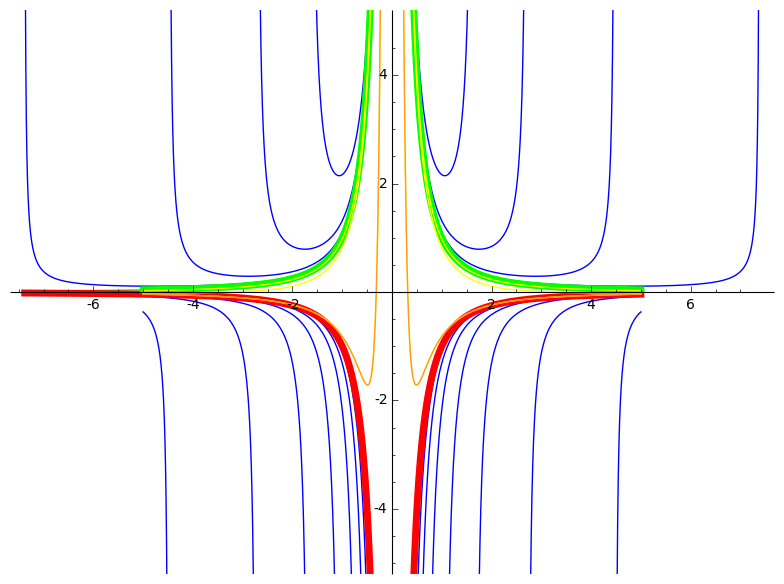
\includegraphics[scale=.3]{imagenes/SolGrup.png}
\caption{Soluciones de  $y'=xy^2-\frac{2y}{x}-\frac{1}{x^3}$}\label{fig:sol_met_lie}
\end{center}
\end{wrapfigure}
Como sabíamos que debía suceder el resultado del segundo miembro no depende sólo de $r$. Integrando
\[s=\frac12\ln\left( \frac{r-1}{r+1}  \right)+C.\]
Sustituyendo
\[\ln|x|=\frac12\ln\left( \frac{x^2y-1}{x^2y+1}  \right)+C.\]
Despejando
\begin{equation}\label{eq:sol_ejem}y =-\frac{x^2 + C}{x^2(x^2 - C)}\end{equation}
La ecuación característica reducida \eqref{eq:sol_inv} es para la ecuación de este ejemplo:
\[0=\overline{Q}=-2y- \left(xy^2-\frac{2y}{x}-\frac{1}{x^3}  \right)x=-x^2y^2+\frac{1}{x^2}\]
Cuyas soluciones son
\[y=\pm\frac{1}{x^2}.\]
Que además son solución de la ecuación diferencial. La curva $y=-1/x^2$ se obtiene de \eqref{eq:sol_ejem} con $C=0$. La  curva $y=-1/x^2$. En la figura \ref{fig:sol_met_lie} graficamos las distintas soluciones.Las curvas azules y naranjas se corresponden con las gráficas de \eqref{eq:sol_ejem} con $c>0$ y $c<0$ respectivamente. La verde es la de $y=1/x^2$ y la roja de $y=-1/x^2$.









\begin{ejemplo} Resolver
\[y'=\frac{y+1}{x}+\frac{y^2}{x^3},\quad x\neq 0,\]
sabiendo que la ecuación es invariante para el grupo de simetrías
\[(\hat{x},\hat{y})=\left(\frac{x}{1-\epsilon x},\frac{y}{1-\epsilon x}   \right).\]
\end{ejemplo}
Ya hemos computado las coordenadas canónicas en la subsección \ref{pag:can_ejem_p}:
\[(r,s)=\left(\frac{y}{x},\frac{1}{x}\right).\]
Por \eqref{eq:prin_en_canon} la ecuación se escribe
\[\frac{dr}{ds}=\frac{-\frac{1}{x^2} }{-\frac{y}{x^2}+\frac{1}{x}\left(
\frac{y+1}{x}+\frac{y^2}{x^3}\right)}=\frac{1}{1+r^2},\]
cuya solución es
\[s=\arctan(r)+C\Rightarrow y=-x\tan\left(\frac{1}{x}+C\right).\]



\subsection{Ecuaciones homogéneas}
\begin{ejemplo} En este ejemplo deduciremos nuevamente el método de solución de ecuaciones homogéneas apelando a las simetrías. Es decir, queremos resolver la ecuación
\boxedeq{y'=F\left(\frac{y}{x}\right).}{eq:homogenea}
\end{ejemplo}
Aquí tenemos el Grupo de Lie de simetrías de cambio de escalas
\[(\hat{x},\hat{y})=(e^{\epsilon}x,e^{\epsilon}y).\] 
Por los resultados de la subsección \ref{pag_ejem_canon1}, $(r,s)=(y/x,\ln|x|)$ son canónicas y la ecuación se escribe
\[\frac{ds}{dr}=\frac{\frac{1}{x}}{-\frac{y}{x^2}+\frac{F\left(\frac{y}{x}\right)}{x}}=\frac{1}{F(r)-r}.\]
La solución general es 
\[\ln|x|=\int^{y/x}\frac{dr}{F(r)-r}+c.\]




\subsection{Método de Lie y \texttt{SymPy}}
\text{SymPy} Incorpora distintas estrategías para resolver ecuaciones por el método de Lie. Hay mucho por indagar al respecto, pero sólo vamos a mencionar una función para calcular los infinitesimales $(\xi,\eta)$.  Aprovechamos para mostrar como luce una consola de \texttt{ipython}, otra manera de usar \texttt{Python} y \texttt{SymPy}.

\begin{lstlisting}
In [1]: from sympy import *
In [2]: init_printing()
In [3]: x=symbols('x')
In [4]: y=Function('y')(x)
In [5]: from sympy.solvers.ode import infinitesimals
In [6]: infinitesimals((y+1)/x+y**2/x**3-y.diff(x))
Out[6]: 
\end{lstlisting}

\[\left [ \left \{ \eta{\left (x,y{\left (x \right )} \right )} : x y{\left (x \right )}, \quad \xi{\left (x,y{\left (x \right )} \right )} : x^{2}\right \}\right ]\]



\section{Diagrama conceptual}

\begin{center}
 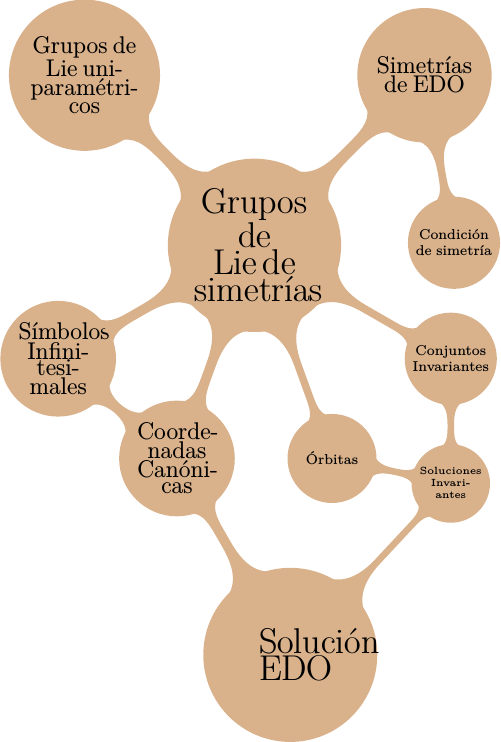
\includegraphics[scale=.25]{imagenes/diagrama.png}
\end{center}


\begin{subappendices}
 

\section{Formas Diferenciales, una introducción ingenua}\label{section:fromas}





 La  expresión \eqref{eq:gral_orden1} es más asimétrica, entre las variables $x$ e $y$ una de ellas es independiente ($x$) y la otra independiente  ($y$).  La expresión \eqref{eq:gral_orden1_FormDif}  es  más simétrica, las dos variables tienen el mismo estatus.

 Las expresiones del tipo \eqref{eq:gral_orden1_FormDif} representan un ente matemático importante llamado \href{http://es.wikipedia.org/wiki/Forma_diferencial}{forma diferencial}\link. No disponemos del tiempo necesario para dotar con entidad matemática el concepto de forma diferencial. Tampoco  resulta de vital importancia. Pero las reglas que rigen la combinación de las formas diferenciales son muy simples y nos gustaría describir este aspecto de las formas diferenciales brevemente; como motivación para un estudio posterior más profundo y para que el lector gane en confianza en su manipulación. Daremos así una pintura de las formas diferenciales incompleta, por cuanto sólo diremos como ellas se combinan pero no contestaremos la pregunta de que son. Sólo digamos, para advertir al lector sobre los requisítos teóricos que se requieren, que las formas diferenciales se encuentran asociados al concepto de variedad diferencial, concepto este que generaliza al de curva y superficie.  Más 
concretamente, las formas diferenciales son funciones que toman valores en los duales de los espacios tangentes a las variedades diferenciales. En particular hay formas diferenciales asociadas a los espacios euclideo, que podemos identificar con  $\rr^n$.

Aqui vamos a pensar a las formas diferenciales como objetos puramente formales sobre los que actúa un operador $d$, leyes de composición internas y externas. Se construyen formas diferenciales invocando un sistema de coordenadas $x_1,\ldots,x_n$. Estas coordenadas, deben ser coordenadas de alguna variedad diferencial, pero, por simplicidad, supondremos que son coordenadas cartesianas ortogonales de un espacio euclideo. Las formas diferenciales forman un espacio vectorial con una operación de suma $+$ y producto por un escalar. Además tienen definido un producto $\wedge$, llamado \href{https://es.wikipedia.org/wiki/Producto_exterior}{producto exterior}\link, que posee  algunas particularidades.  Como los polinomios, las formas diferenciales tienen grado. Por eso se dice que forman un álgebra graduada. A diferencia de los polinomios, este grado no supera la dimensión $n$ del espacio ($\rr^n$ o más generalmente una variedad) a la que están asociadas. Para ser más exactas, la única forma 
de 
grado $k>n$ es la trivial, esto es la nula. Denotamos $\Lambda_k$ las formas de grado $k$, siendo $\Lambda =\bigoplus_{k=0}^{n}\Lambda_k$ el espacio vectorial de todas ellas. Luego $d:\Lambda\to\Lambda$ y $\wedge:\Lambda\times\Lambda\to \Lambda$. Ahora describimos unas simples reglas de las formas,  $d$ y $\wedge$.



\begin{enumerate}
   \item Una 0-forma diferencial es una función $g(x_1,\ldots,x_n)$.

  \item Si $\alpha\in\Lambda_k$ y $\beta\in\Lambda_p$ entonces $\alpha \wedge \beta\in \Lambda_{k+p}$.
  \item El producto $\wedge$ es asociativo, distributivo y satisface una especia de anticonmutatividad, especídficamente si $\alpha\in\Lambda_k$ y $\beta\in\Lambda_p$ entonces $\alpha\wedge \beta=(-1)^{kp}\beta\wedge\alpha$. En particular $\alpha\wedge\alpha=0$ cuando $\alpha$ es un $k$-forma con $k$ impar.
  \item El diferencial satisface
  \begin{enumerate}
    \item Si $\omega$ es una $k$-forma diferencial $d\omega$ es una $k+1$ forma diferencial.
    \item  $d^2\omega=d(d\omega)=0$, para toda $\omega\in\Lambda$.
    \item Si $\alpha\in\Lambda_k$ entonces  $d(\alpha\wedge\beta)=d\alpha\wedge\beta+(-1)^k\alpha\wedge d\beta$.
    \item En el caso de $0$-forma (función) $g(x_1,\ldots,x_n)$ el diferencial se define
    \[dg=\frac{\partial g}{\partial x_1}dx_1+\cdots+\frac{\partial g}{\partial x_n}dx_n\]

  \end{enumerate}
  \item Las expresiones $dx_i$, $i=1,\ldots,n$ forman una especie de base del espacio de las formas $\Lambda$, en el sentido que cualquier $k$ forma $\alpha$ se expresa de la siguiente manera:
  \[\alpha=\sum_{1\leq i_1<\cdots i_k\leq n}g_{i_1\ldots i_k} dx_{i_1}\wedge\cdots\wedge dx_{i_n},\]
  para ciertas funciones $g_{i_1\ldots i_k}$. Observar que la suma se extiende sobre todos los subconjuntos ordenados de $\{1,\ldots,n\}$.
\end{enumerate}


Una $k$-forma diferencial $\alpha$ se llama \href{https://es.wikipedia.org/wiki/Formas_diferenciales_cerradas_y_exactas}{exacta}\link cuando es el diferencial de una $k-1$-forma y se dice \href{https://es.wikipedia.org/wiki/Formas_diferenciales_cerradas_y_exactas}{cerrada}\link cuando $d\alpha=0$. Las propiedades de las formas implican que toda forma exacta es cerrda. Un famoso \href{https://es.wikipedia.org/wiki/Formas_diferenciales_cerradas_y_exactas#Lema_de_Poincar.C3.A9}{Lema de Poincare}\link trata con el recíproco de esta afirmación.

Las reglas anteriores permiten computar cualquiera de las operaciones.
\begin{ejemplo} Si $\alpha=M(x,y)dx+N(x,y)dy$ es una 1-forma de $\rr^2$, entonces
\[ \begin{split}
    d\alpha&=dM\wedge dx-Md^2x + dN\wedge dy-Nd^2y\\
    &=\left(\frac{\partial M}{\partial x}dx+ \frac{\partial M}{\partial y}dy\right)\wedge dx+
    \left(\frac{\partial N}{\partial x}dx+ \frac{\partial N}{\partial y}dy\right)\wedge dy\\
    &= \left(\frac{\partial N}{\partial x}- \frac{\partial M}{\partial y}\right) dx\wedge dy
   \end{split}
\]
Recordemos el famoso \href{https://es.wikipedia.org/wiki/Teorema_de_Green}{Teorema de Green}\link, que afirmaba que si $D\subset \rr^2$ era una región cuyo borde $C=\partial D$ era una curva cerrada simple, entonces
\[\ointctrclockwise_{\partial D} Mdx +Ndy=\iint_D \left(\frac{\partial N}{\partial x}- \frac{\partial M}{\partial y}\right) dx dy.\]
Utilizando formas diferenciales este resultado se escribe de la manera, mucho más compacta y sugerente
\[\ointctrclockwise_{\partial D} \alpha = \iint_Dd\alpha,\]
donde $\alpha =M(x,y)dx+N(x,y)dy$.  Esto es una relación clave de las formas diferenciales que se generaliza en un teorema fundamental de la matemática llamado \href{https://es.wikipedia.org/wiki/Teorema_de_Stokes}{Teorema de Stokes}\link.
\end{ejemplo}




\begin{ejemplo} Computemos $d^2g$, cuando $g$ es una función (0-forma).

\[
\begin{split}
d^2g&=d\left(\frac{\partial g}{\partial x_1}dx_1+\cdots+\frac{\partial g}{\partial x_n}dx_n\right)\\
&= d\left(\frac{\partial g}{\partial x_1}\right)\wedge dx_1+\cdots+d\left(\frac{\partial g}{\partial x_n}\right)\wedge dx_n
    -\frac{\partial g}{\partial x_1}\wedge d^2x_1-\cdots-\frac{\partial g}{\partial x_n}\wedge d^2x_n\\
    &=\left(\sum_{i=1}^n\frac{\partial^2g}{\partial x_i\partial x_1} dx_i\right)\wedge dx_1+\cdots+\left(\sum_{i=1}^n\frac{\partial^2g}{\partial x_i\partial x_n} dx_i\right)\wedge dx_n\\
    &= \sum_{i\neq 1}^n\frac{\partial^2g}{\partial x_i\partial x_1} dx_i\wedge dx_1+\cdots
    \sum_{i\neq n}^n\frac{\partial^2g}{\partial x_i\partial x_n} dx_i\wedge dx_n\\
    &=\sum_{1\leq i<j\leq n}^n\left\{\frac{\partial^2g}{\partial x_i\partial x_j}- \frac{\partial^2g}{\partial x_j\partial x_i}\right \} dx_i\wedge dx_j=0.
\end{split}
\]
Que es lo que tenía que ser.


\end{ejemplo}

\section{Formas diferenciales en Sympy}

En este apéndice resolveremos el problema planteado en el ejemplo \ref{ej:cambio_forma} usando formas diferenciales y Sympy.  Usaremos el módulo de geometría diferencial, donde se pueden definir formas diferenciales
y otros entes propios de la geometría diferencial: campos escalares  y
vectoriales. No es posible entender completamente este módulo sin introducir conceptos básicos de geometría diferencial, cosa que no haremos pues nos alejaría del propósito del curso. De modo que vamos a discutir superficialmente la solución de este problema.  Es suficiente importar del módulo de geometría diferencial el submodulo R2, que ya nos
crea las formas diferenciales $dx$, $dy$  (se accede por \texttt{R2.dx}, \texttt{R2.dy}), como
así también las formas $dr$ y $d\theta$ (\texttt{R2.dr}, \texttt{R2.dtheta}). Tecnicamente hablando R2 es una variedad diferencial --en este caso el espacio euclideano bidimensional-- con toda la estructura algebraica que lleva consigo.

En el siguiente código, luego de las sentencias de importanción, cada línea efectúa lo siguiente: 4-define la forma diferencial en coordenadas cartesianas, 5 y 6-calcula el valor de M y N en coordenadas polares --$Md\theta+N dr$--. Sin embargo el resultado, todavía tiene apelaciones a las coordenadas $x$ e $y$. Por este motivo en las líneas 7 y 8 introducimos los símbolos $r$ y $theta$ y en las líneas 9 a 11 sustituímos $x$ e $y$ por $r\cos\theta$ y $r\sen\theta$ respectivamente. Hay que notar que los simbolos que introdujimos $r$ y $\theta$ son diferentes de \texttt{R2.theta} y \texttt{R2.r}, a los que sympy despliega en negritas en la consola de ipython.  Por ese motivo, también sustituímos   \texttt{R2.theta} y \texttt{R2.r} por $\theta$ y $r$ respectivamente.

 \lstinputlisting[language=Python]{scripts/sust_formas.py}
\marginpar{
\begin{pspicture}(0,-2)(1in,1in)
      %\rput(0,1){
      \scalebox{.5}{\psbarcode[file]{scripts/sust_formas.py}{}{qrcode}}
      %}
\end{pspicture}
}

La forma obtenida es $-rdr+(-r^4+r^2)d\theta$.




\section{Teoría de grupos computacional: GAP}


\begin{quote}
 <<
GAP (Groups, Algorithms, Programming) es un sistema de álgebra discreta computacional, con especial énfasis en la teoría de grupos computacional. GAP proporciona un lenguaje de programación, una biblioteca de miles de funciones implementando algoritmos algebraicos escritos en el lenguaje GAP, así como bibliotecas de datos de objetos algebraicos de gran tamaño [...] GAP se utiliza en la investigación y la enseñanza para estudiar grupos y sus representaciones, anillos, espacios vectoriales, álgebras, estructuras combinatorias, y más. El sistema, incluida la fuente, se distribuye libremente.>>
\end{quote}
\begin{flushright}
 \href{https://www.gap-system.org/}{(Página Oficial de GAP)}\link
\end{flushright}

Hasta donde sabemos Sympy no implementa objetos de teoría de grupos. Sin embargo existe software libre para estudiar grupos. El más conocido de ellos es GAP. Este sistema provee un lenguaje muy sencillo y transparente. Lamentablemente el estudio de esta herramienta está más allá de los alcances de este documento. Desarrollemos un simple ejemplo.

\begin{ejemplo} En el siguiente ejemplo de sesión con línea de comandos de GAP introducimos sentencias que quedan indicadas en cada línea iniciada con el símbolo de sistema (prompt) \verb~>gap~. Las líneas que no inician con el símbolo de sistema indican la salida correspondiente a la sentencia que antecede dichas líneas. En línea 1 introducimos el grupo simétrico de orden 3 y lo llamamos \texttt{G}. En línea 3 pedimos que nos enumere los elementos de \texttt{G}. En línea 5, introducimos el elemento de \texttt{G} que en notación cíclica se escribe $(1,3,2)$. En líneas 7 y 9 calculamos potencias de \texttt{r}. En 11 definimos como \texttt{H} el subgrupo generado por
\texttt{r} y en 13 enumeramos los elementos de \texttt{H}. En 15 averiguamos si \texttt{H} es normal. Siendo este el caso, podemos calcular el grupo cociente en 17 y lo llamos \texttt{K}. Por último averiguamos el orden de \texttt{K} en 19.


\end{ejemplo}
\lstinputlisting[language=GAP]{scripts/gap_basico.g}



\end{subappendices}
\nocite{*}
  \bibliographystyle{apalike-url}
  \bibliography{Grupos_Simetrias.bib}


%\end{document}

